\documentclass{article}

\usepackage{amssymb}
\usepackage[table,xcdraw]{xcolor}
\usepackage{amsmath}
\usepackage[brazilian]{babel}
\usepackage[utf8x]{inputenc}
\usepackage[sc]{mathpazo} 
\linespread{1.05}
\usepackage{microtype}
\usepackage[hang, small,labelfont=bf,up,textfont=it,up]{caption}
\usepackage{lettrine}
\usepackage{graphicx}
\usepackage{gnuplottex}
\usepackage{epstopdf}
\usepackage{multicol}
\usepackage{multirow}
\usepackage{array}
\usepackage{wrapfig}
\usepackage{svg}

\usepackage[hmarginratio=1:1,top=20mm,bottom=35mm,right=15mm,left=15mm,columnsep=20pt]{geometry}
%\usepackage{multicol} 
\usepackage{booktabs}
\usepackage{float} 
\usepackage{subfigure}
\usepackage{paralist} 
\usepackage{hyperref} 
\usepackage{abstract}
\renewcommand{\abstractnamefont}{\normalfont\bfseries}
\renewcommand{\abstracttextfont}{\normalfont\small\itshape}
\usepackage{titlesec}
\renewcommand\thesection{\Roman{section}}
\renewcommand\thesubsection{\Roman{subsection}} 
\titleformat{\section}[block]{\Large\scshape}{\thesection.}{1em}{} 
\titleformat{\subsection}[block]{\large}{\thesubsection.}{1em}{}
\usepackage{verbatim}
\usepackage{fancyhdr} 
\pagestyle{fancy} 
\fancyhead{} 
\fancyfoot{} 

\definecolor{cinzaclaro}{HTML}{84929f}

%AQUI VOCE COLOCA A SIGLA do grupo
\fancyhead[C]{Turma A $\cdot$ Física Experimental V $\cdot$ Bobinas de Helmholtz e Cálculo da Relação Carga/Massa do Elétron $\cdot$ Equipe 5}
\fancyfoot[C]{\thepage} \newenvironment{Figure}
  {\par\medskip\noindent\minipage{\linewidth}}
  {\endminipage\par\medskip}

% AQUI VOCÊ COLOCA O TÍTULO DO SEU EXPERIMENTO.

\title{\vspace{-18mm}\fontsize{16pt}{18pt}\selectfont\textbf{Bobinas de Helmholtz e Cálculo da Relação Carga/Massa do Elétron}} 


% AQUI VOCE COLOCA O NOME DOS AUTORES DO TRABALHO

\author{
\large
\textsc{Jonas Everton Gomes de Araújo\thanks{jonasega@discente.ufg.br }, Sérgio Wilson de Sá Roriz\thanks{sergiodx@discente.ufg.br}, Vinícius Martins Bento\thanks{vinicius\_martinsbento@discente.ufg.br}}\\[2mm]
\large Instituto de Física, Universidade Federal de Goiás \\
%\vspace{2mm}
\large Prof. \textsc{Ricardo Costa de Santana}
}
\date{}

\begin{document}
\maketitle

\thispagestyle{fancy} 
 
%___________________________________

\begin{abstract}
\textbf{Os fenômenos magnéticos são conhecido desde a antiguidade, mas foi a partir do século XIX com Oersted, que tal fenômeno começou a ser estudado em sua integralidade. Em que os experimentos idealizados tiveram por consequência as tecnologias contemporâneas, como equipamentos telecomunicações e de toda a maquinaria elétrica. Dada a importância desta temática, o presente trabalho propõe investigar o campo magnético produzido num arranjo de Bobinas de Helmhotz, com o auxilio de uma sonda Hall, e mensurar a razão carga/massa do elétron, através de um trajetórias circulares originadas em um tubo de raios catódicos no mesmo arranjo.}
\end{abstract}
%
\vspace{0.5cm}

\setlength{\columnsep}{10pt}%
\section{Introdução}

Em determinados casos, é necessário produzir um campo magnético uniforme de baixa intensidade em um volume relativamente grande. Para tal fim, é, em geral, utilizado o equipamento desenvolvido por Hermann Ludwig Ferdinand von Helmholtz (1821-1894), denominado atualmente por \textbf{bobina de Helmholtz}. Esse aparelho consiste de duas bobinas coaxiais circulares separadas por uma distância escolhida cada uma contendo um número $N$ de espiras de raio $R$ com correntes fluindo no mesmo sentido. Veja figura \ref{helmholtz}.

\begin{wrapfigure}[18]{r}{0.4\textwidth}
    \centering
    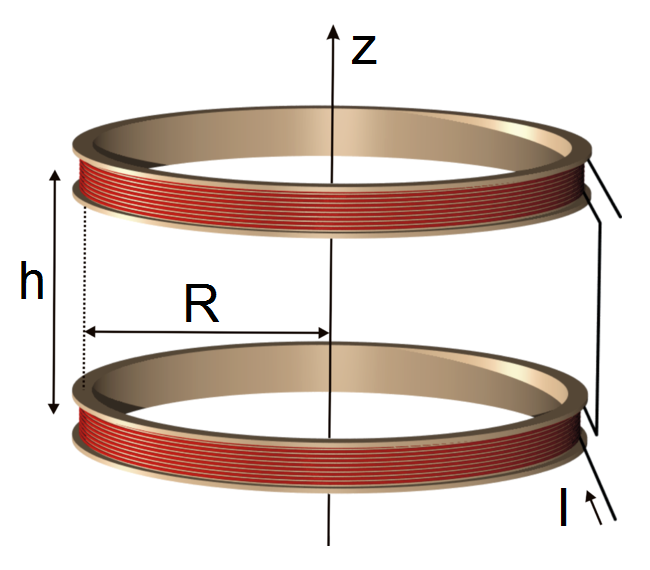
\includegraphics[width=7cm]{./Imagens/Helmholtz.png}
    \caption{Esquematização de uma bobina de Helmholtz. }
    \label{helmholtz}
\end{wrapfigure}

As aplicações da bobina de Helmholtz são várias, por exemplo: determinação das componentes vertical e horizontal do campo magnético terrestre, bem como sua anulação em determinado volume; calibração de medidores de campo magnético de baixa frequência; estudo dos efeitos de campos magnéticos em componentes ou equipamentos eletrônicos; medidas de susceptibilidade magnética; calibração de equipamentos de navegação; estudo de efeitos biomagnéticos; ajuste de tubos de raios catódicos; estudo da performance de tubos de fotomultiplicadoras em campos magnéticos; medidas de magnetorresistência; desmagnetização de pequenas peças de materiais ferromagnéticos usados na ciência de naves espaciais. Nesse experimento, ela foi usada para a determinação da carga específica do elétron.

Para entender o funcionamento de uma bobina de Helmholtz, deve-se lembrar que o campo magnético formado por uma bobina circular é dado por:

\begin{equation}
    \label{biotsavartequation}
    d \vec B =  \frac{\mu _0 I}{4 \pi} \frac{d \vec l \times \vec \rho} {\rho ^3}
\end{equation}
onde $\mu _0$ é permeabilidade magnética do vácuo, $\vec \rho$ é o vetor que vai do elemento condutor $d \vec l$ até ponto de de medida $\vec B$, e $d \vec B$ é perpendicular ao vetores $\vec \rho$ e $d \vec l$. Veja a figura \ref{biotsvartimage}.

\begin{wrapfigure}[15]{r}{0.4\textwidth}
    \centering
    \includesvg[width=7.4cm]{./Imagens/SpireCourant.svg}
    \caption{Esquema demonstrando a direção e sentido dos vetores presentes na Lei de Biot-Savart (eq. \ref{biotsavartequation}). }
    \label{biotsvartimage}
\end{wrapfigure}

Como o vetor $d \vec l$ é perpendicular aos vetores $\vec \rho$ e $d \vec B$ e ainda perpendicular ao plano da figura, enquanto os outros dois vetores estão no plano da figura, a equação \ref{biotsavartequation} pode ser reescrita como:

\begin{equation}
    dB = \frac{\mu _0 I}{4 \pi} dl = \frac{I}{4 \pi} \frac{\mu _0 dl}{R^2 +z^2}
\end{equation}

sendo $z$ a distância do centro da espira ao ponto onde estamos calculando o campo. Como mostrado na figura, $dB$ pode ser dividido em duas componentes, uma radial $dB$ e uma axial $dB _z$ . Para qualquer elemento $dl$ que escolhermos na espira a componente $dB _z$ do campo terá sempre a mesma direção, podendo, portanto serem somadas, já as componentes $dB _r$ se anulam aos pares. Sendo assim o campo na direção radial é nulo, ou seja, $\mathbf{B _r = 0}$ e o campo ao longo da direção $z$ (axial) é dado por:

\begin{equation}
    \label{bz}
    B _z = \frac{\mu _0 I}{2}\frac{R^2}{(R^2 + z^2)^{\frac{3}{2}}} =  \frac{\mu _0 I}{2R}\frac{1}{(1 + (z/R)^2)^{\frac{3}{2}}}
\end{equation}

O campo magnético de uma bobina circular de $N$ espiras é então obtido multiplicando-se o número de espiras pela equação (\ref{bz}). Dessa forma, o campo ao longo do eixo das duas bobinas idênticas a uma distância a do centro das bobinas é:

\begin{equation}
    \label{bzn}
    B(z,r=0) =  \frac{\mu _0 I N}{2R} \left [ \frac{1}{(1 + A^2)^{\frac{3}{2}}} + \frac{1}{(1 + A'^2)^{\frac{3}{2}}} \right ]
\end{equation}
Com
\begin{equation*}
    A = \frac{z-a/2}{R} \qquad e \qquad A' = \frac{z+a/2}{R}     
\end{equation*}

Quando  $z = 0$, o campo magnético tem um valor máximo para $a < R$ e mínimo para $a > R$. A dependência de $B$ com a posição ao longo do eixo axial das bobinas é virtualmente uniforme para o intervalo $\frac{-R}{2} < z < \frac{R}{2}$, quando $a = 0$. O campo $B$ no ponto médio entre as bobinas quando a separação a entre elas for igual ao raio $R$ é:

\begin{equation}
    \label{b0}
    B(0,0) = \frac{\mu _0 I N }{2R} \frac{2}{(5/4)^{\frac{3}{2}}} = 0,716 \mu _0 N \frac{I}{R}
\end{equation}
onde escolhemos como origem do sistema de coordenadas o ponto médio entre as bobinas sobre o eixo axial, para uma bobina com N = 154 espiras, raio R = 20 cm e corrente I = 4,0 A, o valor do campo B é de:

\begin{equation}
    B(0,0) = 2,77 \ mT
\end{equation}

Em 1897, Joseoh John Thomson(1856-1940) calculou a relação entre a carga elétrica e a massa do elétron, usando como aparato a bobina de Helmholtz. Esses experimento lhe valeu o Prêmio Nobel da Física, em 1906. Para isso, Thomson usou uma ideia simples: se um portador de carga elétrica estiver se movendo em um campo magnético perpendicular à sua velocidade, então o portador de carga sofrerá uma deflexão em sua trajetória.

A força magnética $\vec F$  que age sobre um portador de carga $q$ que se movimenta com velocidade $\vec v$ num campo magnético $\vec B$ é dada pela relação vetorial apresentado abaixo:

\begin{equation}
    \vec F  = q \cdot ( \vec v \times \vec B)
\end{equation}

Se o portador de carga tem uma velocidade perpendicular ao campo magnético gerado pelas bobinas $(\vec v \perp \vec B)$, então a Força de Lorentz apresentado acima se reduz à da equação \ref{v1}, que mostra como fica estabelecida a velocidade do portador de carga $v$ quando a Força Magnética atua como Força Centrípeta no feixe de elétrons:

\begin{equation}
    \label{v1}
    v= \frac{q}{m _0}Br
\end{equation}
sendo $m _0$ a massa do portador de carga.

Quando um portador de carga $q$ e de massa $m _0$ é acelerado por diferença de potencial $U$, sua energia cinética é dada pela equação \ref{energia} abaixo

\begin{equation}
    \label{energia}
    q \cdot U = \frac{1}{2} mv^2
\end{equation}

Se $v$ é a norma da velocidade do portador de carga apresentada na equação \ref{v1}, então, chegamos na relação carga/massa:

\begin{equation}
    \label{qm}
    \frac{q}{m _0}= \frac{2U}{(Br)^2}
\end{equation}

\section{Descrição experimental}

\begin{wrapfigure}[15]{r}{0.4\textwidth}
    \centering
    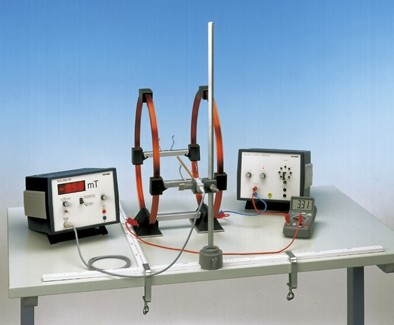
\includegraphics[width=7cm]{Imagens/Experimento 2.1.png}
    \caption{Aparato experimental para a primeira etapa.}
    \label{1etapa}
\end{wrapfigure}

O experimento executado em laboratório divide-se em duas partes: na primeira parte, consisti em mapear o campo magnético gerado por um par de bobinas circulares planas para verificar a uniformidade do campo magnético na área relativamente grande entre as bobinas; na segunda parte, envolve o uso desse arranjo para determinar a relação carga/massa do elétron com base na trajetória do feixe de elétrons observada produzida pelo tubo de raios catódicos.

\subsection{Primeira Etapa}

Para a primeira parte, utiliza-se uma fonte de corrente contínua, duas bobinas circulares, um multímetro, uma sonda Hall, réguas e um teslâmetro. Veja figura \ref{1etapa} que mostra todo o aparato experimental.

Primeiro, as bobinas foram conectadas em série, de modo que a corrente contínua fluísse por elas na mesma direção. A corrente utilizada foi de 4,0 A. Em seguida, a sonda Hall já preso em um suporte com base móvel, foi nivelada e alinhada com o eixo das bobinas. Com ajuda das réguas fixadas ao balcão, as bobinas foram postas à uma distância $a = 2R$ uma da outra, onde R corresponde ao raio das bobinas. Com a corrente circulando, a sonda Hall foi movimentada de 1 em 1 cm na direção radial. Logo depois, repetiu-se o experimento para $a=R$ e $a=R/2$

Após isso, foram repetidos esses mesmos experimentos mas agora na direção axial.

\subsection{Segunda Etapa}

\begin{wrapfigure}[10]{r}{0.4\textwidth}
    \centering
    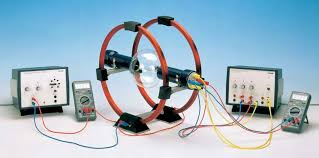
\includegraphics[width=7cm]{Imagens/Experimento 2.2.png}
    \caption{Aparato experimental da segunda etapa.}
    \label{2etapa}
\end{wrapfigure}

Para a primeira parte, utiliza-se um par de bobinas circulares, dois multímetros, um tubo de raios catódicos e duas fontes que pode ser visto na figura \ref{2etapa} que tem por objetivo calculara a razão carga/massa do elétron. Apagou-se as luzes da sala e as fontes foram ligadas aparecendo um feixe curvo luminescente no interior do tubo. Variando a corrente das bobinas, a intensidade do campo magnético muda, e pela equação (\ref{qm}), alteramos, assim, o raio da órbita dos elétrons. Variou-se a corrente de forma a se fazer o feixe coincidir com os traços luminosos no interior do tubo, quando esse evento ocorria, somente metade do círculo era observado. As medições das correntes foram feitas para os raios de trajetória de 2, 3, 4 e 5 cm. 

\section{Resultados e Discussão}

\subsection{Primeira Etapa}

Seguindo o procedimento experimental foi aplicada uma corrente $I = 4,0 A$ nas bobinas
circulares de raio $R = 20 cm$ com 154 espiras. Primeiramente, foram realizadas medições para
a componente radial do campo magnético em três configurações distintas, utilizando $a = 2R$,
$a = R$ e, então, $a = R/2$. Após isso, foram realizadas as medições para a componente axial
do campo magnético com as mesmas configurações para o eixo radial, ou seja, utilizando os
mesmos valores do parâmetro $a$. 

Com os dados em mãos, que se encontra na tabela \ref{tabbh} (veja o apêndice), pode-se plotar o gráfico do módulo do campo magnético axial em função da distância. A partir dele, podemos observar a dependência espacial do campo magnético axial, para $a = R/2$, o módulo do campo magnético varia mais significativamente com a distância, ao ponto que para $a = R$ a região onde o campo é constante é maior. Agora para $a = 2R$, o campo tem um valor máximo nas proximidades de uma das bobinas, passando por um mínimo na distância media entre elas e depois aumentando novamente quando nos aproximamos da bobina oposta.

Com os dados obtidos e utilizando a equação (\ref{bzn}), pode-se construir um gráfico com uma previsão teórica para tais valores, essa comparação pode ser vista na figura (\ref{grafbza}).

\begin{figure}[H]
    \centering
    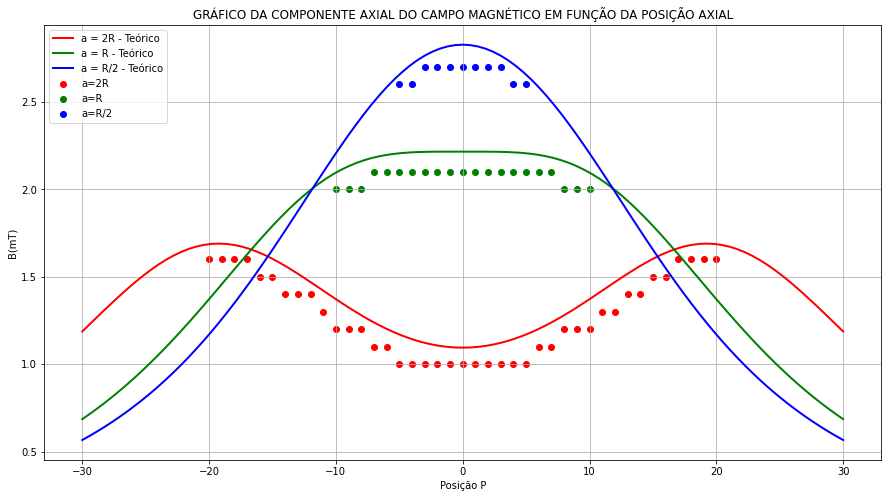
\includegraphics[width=18cm]{Imagens/ga.png}
    \caption{Gráfico da componente axial do campo magnético em função da posição axial}
    \label{grafbza}
\end{figure}

Novamente, com os dados que constam na tabela \ref{tabbh} (veja o apêndice), plotamos o gráfico do módulo do campo magnético radial em função da distância. Vemos que, para $a=R/2$, podemos observar uma parábola com concavidade voltada para cima, onde o valor mínimo do campo encontra-se na distância média, e, também, pode-se observar que próximo aos pontos -14 e 14, há um pico do campo magnético. Para $a=R$ o campo mantém-se na sua maior parte constante e nas extremidades ele decresce (sendo o valor mínimo nas suas extremidades). Agora, para $a=2R$, a curva lembra uma parábola com concavidade para baixo, mostrando que há um valor máximo na origem, e gradualmente o campo diminui quando afastamos a sonda em direção das bordas da bobinas.


\begin{figure}[H]
    \centering
    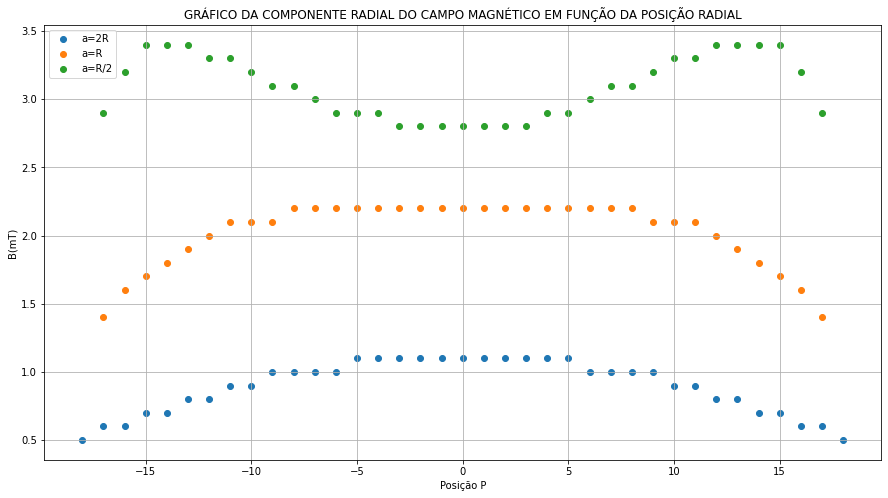
\includegraphics[width=18cm]{Imagens/gr.png}
    \caption{Gráfico da componente radial do campo magnético em função da posição radial}
    \label{grafbzr}
\end{figure}

\subsection{Segunda Etapa}

As correntes medidas para cada raio e tensão, possibilitaram por meio das equações (\ref{b0}) e (\ref{qm}), calcular a razão carga/massa do elétron $\left ( \frac{e}{m _0}\right )$. Os valores para cada medição estão expostos na Tabela \ref{tabqm}. Com a análise dos dados, o valor médio obtido para a razão foi de $(1,68 \pm 0,09) \times 10 ^{11} A \cdot s/kg$, onde a incerteza é dada pelo desvio padrão das medições. A média obtida é bem próxima ao valor teórico de $1,759 \times 10 ^{11} A \cdot s/kg$.

\begin{table}[hb]
\centering
\begin{tabular}{|c|c|c|c|c|c|c|c|c|}
\hline
                                 & \multicolumn{2}{c|}{\cellcolor[HTML]{9B9B9B}\textbf{$\mathbf{R=0,02 \ m}$}}                                                                    & \multicolumn{2}{c|}{\cellcolor[HTML]{9B9B9B}\textbf{$\mathbf{R=0,03 \ m}$}}                                                                    & \multicolumn{2}{c|}{\cellcolor[HTML]{9B9B9B}\textbf{$\mathbf{R=0,04 \ m}$}}                                                                    & \multicolumn{2}{c|}{\cellcolor[HTML]{9B9B9B}\textbf{$\mathbf{R=0,05\ m}$}}                                                                    \\ \cline{2-9} 
\multirow{-2}{*}{\textbf{U (V)}} & \cellcolor[HTML]{EFEFEF}\textbf{I (A)} & \cellcolor[HTML]{EFEFEF}\textbf{$\mathbf{\frac{e}{m} \times 10^{11} \left ( \frac{As}{kg} \right)}$} & \cellcolor[HTML]{EFEFEF}\textbf{I (A)} & \cellcolor[HTML]{EFEFEF}\textbf{$\mathbf{\frac{e}{m} \times 10^{11} \left ( \frac{As}{kg} \right)}$} & \cellcolor[HTML]{EFEFEF}\textbf{I (A)} & \cellcolor[HTML]{EFEFEF}\textbf{$\mathbf{\frac{e}{m} \times 10^{11} \left ( \frac{As}{kg} \right)}$} & \cellcolor[HTML]{EFEFEF}\textbf{I (A)} & \cellcolor[HTML]{EFEFEF}\textbf{$\mathbf{\frac{e}{m} \times 10^{11} \left ( \frac{As}{kg} \right)}$} \\ \hline
150                              & 3,07                                   & 1,66                                                                                  & 2,01                                   & 1,72                                                                                  & 1,47                                   & 1,81                                                                                  & 1,15                                   & 1,89                                                                                  \\ \hline
175                              & 3,47                                   & 1,51                                                                                  & 2,26                                   & 1,59                                                                                  & 1,65                                   & 1,67                                                                                  & 1,27                                   & 1,81                                                                                  \\ \hline
200                              & 3,64                                   & 1,57                                                                                  & 2,34                                   & 1,69                                                                                  & 1,73                                   & 1,74                                                                                  & 1,38                                   & 1,75                                                                                  \\ \hline
225                              & 3,87                                   & 1,56                                                                                  & 2,5                                    & 1,67                                                                                  & 1,85                                   & 1,71                                                                                  & 1,47                                   & 1,74                                                                                  \\ \hline
250                              & 4,09                                   & 1,56                                                                                  & 2,65                                   & 1,65                                                                                  & 1,95                                   & 1,71                                                                                  & 1,56                                   & 1,71                                                                                  \\ \hline
275                              & 4,3                                    & 1,55                                                                                  & 2,78                                   & 1,65                                                                                  & 2,05                                   & 1,70                                                                                  & 1,63                                   & 1,73                                                                                  \\ \hline
300                              & 4,5                                    & 1,54                                                                                  & 2,91                                   & 1,64                                                                                  & 2,16                                   & 1,67                                                                                  & 1,71                                   & 1,71                                                                                  \\ \hline
\end{tabular}
\caption{Valores de tensão, corrente e carga/massa do feixe de elétrons com diferentes raios e trajetórias.}
\label{tabqm}
\end{table}

Após isso, fizemos o teste de compatibilidade (\ref{k}) dado abaixo:

\begin{equation}
    \label{k}
    k =\frac{|A-A'|}{\sqrt{\mu _A ^2 + \mu _{A'} ^2}} = \frac{|1,68-1,759|}{\sqrt{0,09^2 + 0^2}} = 0,877
\end{equation}

Como o valor k ficou abaixo de 2,5, então, podemos dizer que o valor obtido experimentalmente é compatível e aproxima-se do teórico. 

\section{Conclusão}
Ao analisar a tabela e os gráficos, vemos que na primeira parte do experimento conseguimos realizar um bom mapeamento do campo magnético gerado pelas bobinas circulares nas três configurações de distância entre elas. No gráfico da componente axial do campo magnético, os pontos se aproximaram bastante do teórico, e a diferença dos pontos com os gráficos deve-se, provavelmente, devido à interferências de outros campos magnéticos externos em sentido contrário, talvez gerados por outros aparelhos eletrônicos no laboratório. Pode-se também ser devido há algum desgaste da sonda Hall que calculou um campo magnético menor do que realmente devia ser obtido.

Na segunda parte da experimentação , obtivemos um valor bastante aproximado para o valor da razão carga-massa do elétron, calculado pela média dos valores correspondentes que é $(1,68 \pm 0,09) \times 10^{11}$. Esse valor aproximou-se bastante do valor teórico que corresponde à  $1,759 \times 10^{11}$. Isso só foi possível concluir com o cálculo do teste de compatibilidade que deu $k=0,877$ que é menor que 2,5.d


\begin{thebibliography}{99}
\bibitem{vuolo1996fundamentos}
    Vuolo, Jos{\'e} Henrique;
    Fundamentos da teoria de erros.
    Editora Blucher.
    1996.
    
\bibitem{taylor}
    Taylor, John R.;
    Introdução à Análise de Erros. O Estudo de Incertezas em Medições Físicas.
    Bookman.
    2012.
    
\bibitem{fisicaexpV}
    Carvalho, J. F; Maia, L. J. Q; Santana, R. C.
    Física Experimental V (Experimentos de Física Moderna).
    Goiânia, 2019.
    
\bibitem{nussenweig}
    H. M. Nussensweig. 
    Curso de Física Básica, Vols. 3 e 4
    Edgard Blücher.
    1997. 
    
\bibitem{reitz}
    J.R. Reitz, F.J. Milford, R.W. Christy.
    Fundamentos da Teoria Eletromagnética.
    Campus Ltda. 
    1982. 

\end{thebibliography}

\newpage
\Large\textsc{{Apêndice}}

\begin{table}[!ht]
\centering
\begin{tabular}{|c|c|c|c||c|c|c|}
\hline
{\color[HTML]{000000} }                                                                                            & \multicolumn{3}{c||}{\cellcolor{cinzaclaro}\textbf{Eixo Radial}}                                & \multicolumn{3}{c|}{\cellcolor{cinzaclaro}\textbf{Eixo Axial}}                                 \\ \cline{2-7} 
\multirow{-2}{*}{{\color[HTML]{000000} \textbf{\begin{tabular}[c]{@{}c@{}}Bobinas\\ de Helmholtz\end{tabular}}}} & \cellcolor[HTML]{EFEFEF}$a=2R$ & \cellcolor[HTML]{EFEFEF}$a=R$ & \cellcolor[HTML]{EFEFEF}$a=R/2$ & \cellcolor[HTML]{EFEFEF}$a=2R$ & \cellcolor[HTML]{EFEFEF}$a=R$ & \cellcolor[HTML]{EFEFEF}$a=R/2$ \\ \hline
Posição (cm)                                                                                                       & $B(mT)$                        & $B(mT)$                       & $B(mT)$                         & $B(mT)$                        & $B(mT)$                       & $B(mT)$                         \\ \hline
-20,00                                                                                                             & $-$                            & $-$                           & $-$                             & 1,60                           & $-$                           & $-$                             \\ \hline
-19,00                                                                                                             & $-$                            & $-$                           & $-$                             & 1,60                           & $-$                           & $-$                             \\ \hline
-18,00                                                                                                             & 0,50                           & $-$                           & $-$                             & 1,60                           & $-$                           & $-$                             \\ \hline
-17,00                                                                                                             & 0,60                           & 1,40                          & 2,90                            & 1,60                           & $-$                           & $-$                             \\ \hline
-16,00                                                                                                             & 0,60                           & 1,60                          & 3,20                            & 1,50                           & $-$                           & $-$                             \\ \hline
-15,00                                                                                                             & 0,70                           & 1,70                          & 3,40                            & 1,50                           & $-$                           & $-$                             \\ \hline
-14,00                                                                                                             & 0,70                           & 1,80                          & 3,40                            & 1,40                           & $-$                           & $-$                             \\ \hline
-13,00                                                                                                             & 0,80                           & 1,90                          & 3,40                            & 1,40                           & $-$                           & $-$                             \\ \hline
-12,00                                                                                                             & 0,80                           & 2,00                          & 3,30                            & 1,30                           & $-$                           & $-$                             \\ \hline
-11,00                                                                                                             & 0,90                           & 2,10                          & 3,30                            & 1,30                           & $-$                           & $-$                             \\ \hline
-10,00                                                                                                             & 0,90                           & 2,10                          & 3,20                            & 1,20                           & 2,0                           & $-$                             \\ \hline
-9,00                                                                                                              & 1,00                           & 2,10                          & 3,10                            & 1,20                           & 2,0                           & $-$                             \\ \hline
-8,00                                                                                                              & 1,00                           & 2,20                          & 3,10                            & 1,20                           & 2,0                           & $-$                             \\ \hline
-7,00                                                                                                              & 1,00                           & 2,20                          & 3,00                            & 1,10                           & 2,1                           & $-$                             \\ \hline
-6,00                                                                                                              & 1,00                           & 2,20                          & 2,90                            & 1,10                           & 2,1                           & $-$                             \\ \hline
-5,00                                                                                                              & 1,10                           & 2,20                          & 2,90                            & 1,00                           & 2,1                           & 2,60                            \\ \hline
-4,00                                                                                                              & 1,10                           & 2,20                          & 2,90                            & 1,00                           & 2,1                           & 2,60                            \\ \hline
-3,00                                                                                                              & 1,10                           & 2,20                          & 2,80                            & 1,00                           & 2,1                           & 2,70                            \\ \hline
-2,00                                                                                                              & 1,10                           & 2,20                          & 2,80                            & 1,00                           & 2,1                           & 2,70                            \\ \hline
-1,00                                                                                                              & 1,10                           & 2,20                          & 2,80                            & 1,00                           & 2,1                           & 2,70                            \\ \hline
0,00                                                                                                               & 1,10                           & 2,20                          & 2,80                            & 1,00                           & 2,1                           & 2,70                            \\ \hline
1,00                                                                                                               & 1,10                           & 2,20                          & 2,80                            & 1,00                           & 2,1                           & 2,70                            \\ \hline
2,00                                                                                                               & 1,10                           & 2,20                          & 2,80                            & 1,00                           & 2,1                           & 2,70                            \\ \hline
3,00                                                                                                               & 1,10                           & 2,20                          & 2,80                            & 1,00                           & 2,1                           & 2,70                            \\ \hline
4,00                                                                                                               & 1,10                           & 2,20                          & 2,90                            & 1,00                           & 2,1                           & 2,60                            \\ \hline
5,00                                                                                                               & 1,10                           & 2,20                          & 2,90                            & 1,00                           & 2,1                           & 2,60                            \\ \hline
6,00                                                                                                               & 1,00                           & 2,20                          & 3,00                            & 1,10                           & 2,1                           & $-$                             \\ \hline
7,00                                                                                                               & 1,00                           & 2,20                          & 3,10                            & 1,10                           & 2,1                           & $-$                             \\ \hline
8,00                                                                                                               & 1,00                           & 2,20                          & 3,10                            & 1,20                           & 2,0                           & $-$                             \\ \hline
9,00                                                                                                               & 1,00                           & 2,10                          & 3,20                            & 1,20                           & 2,0                           & $-$                             \\ \hline
10,00                                                                                                              & 0,90                           & 2,10                          & 3,30                            & 1,20                           & 2,0                           & $-$                             \\ \hline
11,00                                                                                                              & 0,90                           & 2,10                          & 3,30                            & 1,30                           & $-$                           & $-$                             \\ \hline
12,00                                                                                                              & 0,80                           & 2,00                          & 3,40                            & 1,30                           & $-$                           & $-$                             \\ \hline
13,00                                                                                                              & 0,80                           & 1,90                          & 3,40                            & 1,40                           & $-$                           & $-$                             \\ \hline
14,00                                                                                                              & 0,70                           & 1,80                          & 3,40                            & 1,40                           & $-$                           & $-$                             \\ \hline
15,00                                                                                                              & 0,70                           & 1,70                          & 3,40                            & 1,50                           & $-$                           & $-$                             \\ \hline
16,00                                                                                                              & 0,60                           & 1,60                          & 3,20                            & 1,50                           & $-$                           & $-$                             \\ \hline
17,00                                                                                                              & 0,60                           & 1,40                          & 2,90                            & 1,60                           & $-$                           & $-$                             \\ \hline
18,00                                                                                                              & 0,50                           & $-$                           & $-$                             & 1,60                           & $-$                           & $-$                             \\ \hline
19,00                                                                                                              & $-$                            & $-$                           & $-$                             & 1,60                           & $-$                           & $-$                             \\ \hline
20,00                                                                                                              & $-$                            & $-$                           & $-$                             & 1,60                           & $-$                           & $-$                             \\ \hline
\end{tabular}
\caption{Medições do campo magnético radial e axial para diferentes configurações}
\label{tabbh}
\end{table}

\end{document}